\documentclass[addpoints,12pt]{exam}
\pagestyle{empty}
\usepackage{amsmath}
\usepackage{amssymb}
\usepackage{latexsym}
\usepackage[dvips]{graphicx}
\usepackage{enumerate}
\usepackage{amsfonts}
\newcommand{\nl} {\newline}
\newcommand{\normal}{\triangleleft}
\newcommand{\homo}{\simeq}
\newcommand{\R}{\mathbb{R}}
\newcommand{\Z}{\mathbb{Z}}
\newcommand{\Q}{\mathbb{Q}}
\newcommand{\N}{\mathbb{N}}
\newcommand{\C}{\mathbb{C}}
\newcommand{\ov}{\overline}
\newcommand{\E}{\varepsilon}
\newcommand{\F}{\varphi}
\newcommand{\MF}{\mathbb{F}}
\newcommand{\s}{\sqrt}

\newcommand{\vv}[2]{\begin{bmatrix} #1 \\ #2 \end{bmatrix}}
\newcommand{\vvv}[3]{\begin{bmatrix} #1 \\ #2 \\ #3\end{bmatrix}}
\newcommand{\vvvv}[4]{\begin{bmatrix} #1 \\ #2 \\ #3 \\ #4\end{bmatrix}}
\newcommand{\vvvvv}[5]{\begin{bmatrix} #1 \\ #2 \\ #3 \\ #4 \\ #5  \end{bmatrix}}

\everymath{\displaystyle}
\input{../../../AxesFunction}

\def\arraystretch{2}
\setlength\arraycolsep{20pt}
%\renewcommand{\baselinestretch}{1.3}

\begin{document}

~\hfill Student Name: \rule{2in}{.1pt}\\\\
\phantom{.}\hfill PERM: \rule{2in}{.1pt}\\\\
%\phantom{.}\hfill Section Time (e.g. 8am): \rule{2in}{.1pt}\\
Circle the section you ATTEND (if you are enrolled a different section, note which one):
\vskip.15in

\textbf{\begin{tabular}{cccccc}
Kyle: & Tue:8am & Tue:4pm & Tue:7pm\\
David: & Tue:5pm & Tue:6pm\\
Yihan: & Mon:4pm & Mon:5pm & Mon:6pm & Mon:7pm\\
Tom: & Tue:8am & Tue:4pm & Wed:8am\\
Matt: & Tue:5pm & Tue:6pm & Tue:7pm\\
\end{tabular}}
\vskip.25in



%Spring 2011
%Instructor: Stepan Paul
%Circle Your Section:\quad 8AM:Rahul\quad 4PM:Rahul\quad 5PM:Rahul\quad 6PM:Rahul\quad 6PM:Brandon
%\vskip0.5truein

\centerline{\bf \underline {Math 4B, Midterm 2, Spring 2017}}

\centerline{\bf \underline{Version C}}
\vskip0.2in

\underline {Instructions}: Read the instructions for each question carefully. No calculators, cell phones, or other electronic devices are permitted. No notes or textbooks. Academic dishonesty will not be tolerated. Show your work, write legibly, and circle your answers. 

\vspace{.5in}
\centerline{\gradetable}

\vspace{.5in}


\setlength\arraycolsep{2pt}
\def\arraystretch{1.2}

\textbf{I understand UCSB's policies regarding academic dishonesty, and I certify that this test was taken with academic integrity.}
\vspace{.5in}

Sign and date: \rule{5in}{.5pt}

%\medskip
%\medskip \vskip0.25truein
%\vskip0.25truein

%\vspace{0.5in} \large{\centerline{\begin{tabular}{|c|c|c|} \hline
%Problem  & Points & Score
%\\ \hline
% 1 & 25 &     \\ \hline
% 2 & 10 &      \\ \hline
% 3 & 15 &      \\ \hline
% 4 & 10 &      \\ \hline
% Total & 60 &  \\ \hline
%\end{tabular}}}
%}

\newpage
\begin{questions}
 
 \question[10] Find the general solution to the ODE:
 $$y''+4y'+13y=17e^{3t}$$
 
 \newpage
 
 \question[10] Solve the initial value problem:
 
 $$\begin{array}{ccccc}
  x' & = & 7x & + & 4y \\
  y' & = & 4x & + & y
 \end{array},\qquad x(0)=-5,\quad y(0)=5$$
 

 
 \newpage
 
 \question[9] A 10 kg mass is attached to the end of a spring with spring constant $k=90$ N/m.
 
 \begin{parts}
  \part If there is no damping force, at what frequency will the mass naturally oscillate?
  \vfill
  \part If we add a dashpot to the system with a damping constant of $b=100$ N/(m/s), will the system be over-damped or under-damped?
  \vfill
  \part If we keep the damping consant of $b=100$ N/(m/s) from part (b) but replace the spring, what new spring constant $k$ will cause the system to be critically damped?
  \vfill
 \end{parts}
 
 \newpage
 
 \question[9] Consider the non-linear system
 \begin{align*}
  \frac{dx}{dt}&=x+y\\
  \frac{dy}{dt}&=1-x^2
 \end{align*}
 
 \begin{parts}
  \part List all equilibrium points for this system.
  \vfill
 
  \part Shade the part of the phase plane in which both $x$ and $y$ are increasing.
  
  \tickedaxes3333{}
  \vfill
  
  \newpage
  
  \part The graphs of $x(t)$ and $y(t)$ for a solution $\begin{bmatrix}x\\y\end{bmatrix}$ to the system are shown below. Sketch the solution curve in the phase plane.
  
  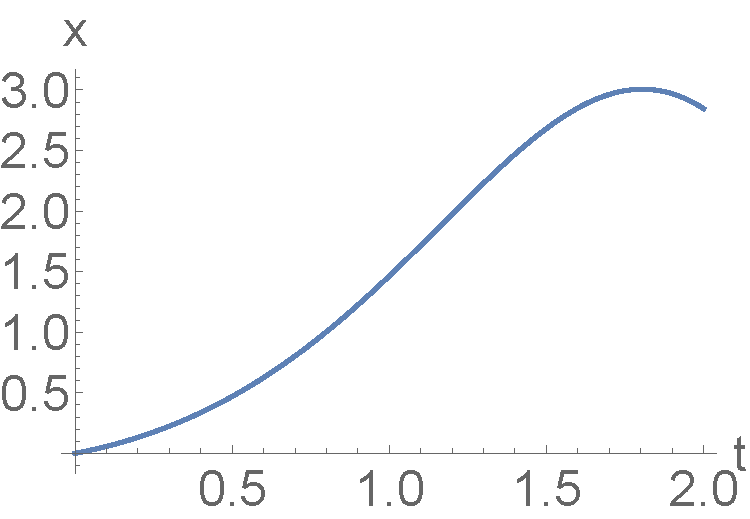
\includegraphics[width=0.4\textwidth]{xtplaneC} \qquad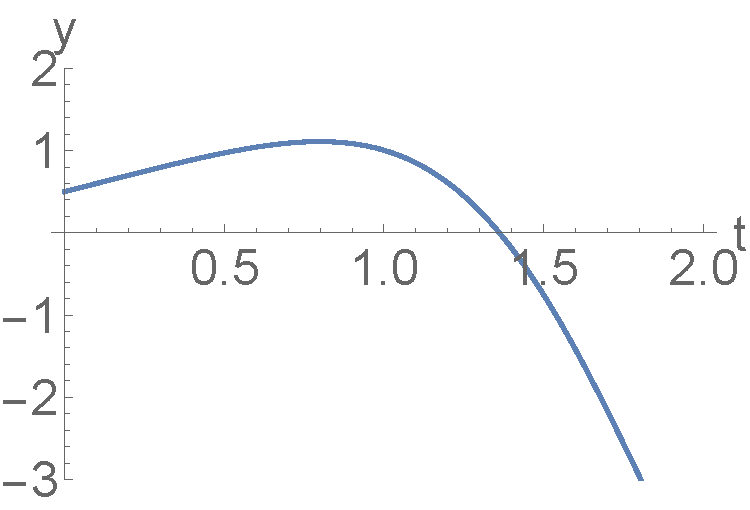
\includegraphics[width=0.4\textwidth]{ytplaneC}
  
  \tickedaxes3333{}
  
 \end{parts}
 
 \newpage
 
 \question[3] The real $2\times2$ matrix $A$  has eigenvector $\vec v_1=\vv{3}{2-i}$ for eigenvalue $\lambda_1=2+i$; and $A$ has eigenvector  $\vec v_2=\vv{3}{2+i}$ for eigenvalue $\lambda_2=2-i$. Given this information, write down the general solution to the system of ODEs
 
 $$\vec x\,'=A\vec x$$
 
 
% \question Squirrels and rabbits both live on the Ellwood bluffs. If $S$ is the number of squirrels (in hundreds), and $R$ is the number of rabbits (in hundreds), their populations are modeled by the non-linear system
% \begin{align*}
%  \frac{dR}{dt}&=0.2R(7-R-0.5S)\\
%  \frac{dS}{dt}&=0.2S(8-S-0.5R)
% \end{align*}
 
 
 
\end{questions}

\newpage

If you finish early, you must stay in your seat until the end. You should check your work, but if you are done, you can amuse yourself by coloring in these regular pentagonal tilings.

\begin{tabular}{cc}
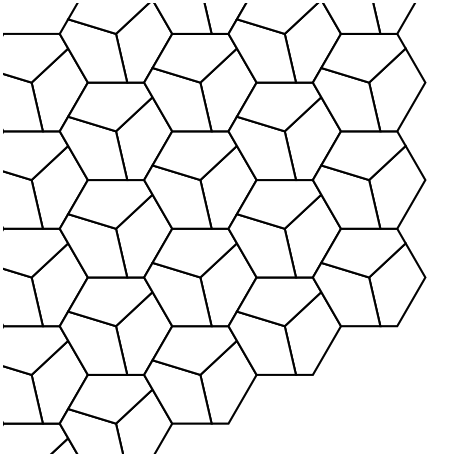
\includegraphics[width=.4\textwidth]{T1} & 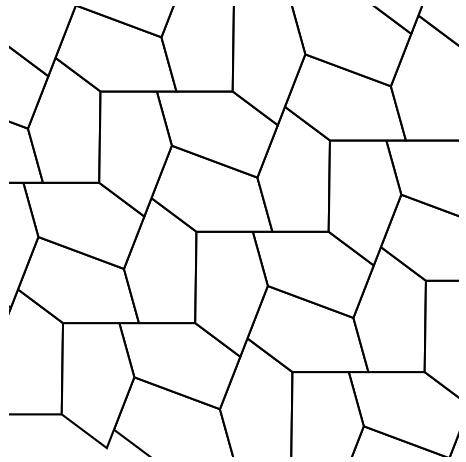
\includegraphics[width=.4\textwidth]{T2} \\
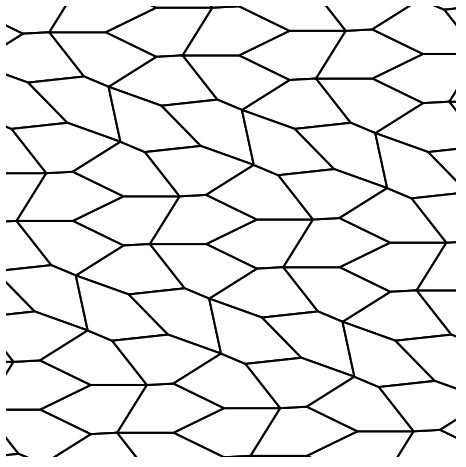
\includegraphics[width=.4\textwidth]{T3} &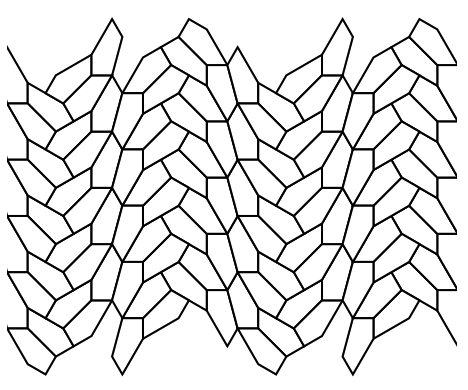
\includegraphics[width=.4\textwidth]{T15} 
\end{tabular}



\end{document}
